\documentclass[11pt]{article}

% Packages
\usepackage{enumitem}
\usepackage{amscd}
\usepackage{amsmath}
\usepackage{amstext}
\usepackage{bbold}
\usepackage{bm}
\usepackage{booktabs}
\usepackage{color}
\usepackage{easybmat}
\usepackage{etex}
\usepackage{framed}
\usepackage[dvips,letterpaper,margin=1in]{geometry}
\usepackage{graphicx}
\usepackage{hyperref}
\usepackage[noabbrev,capitalize]{cleveref}
\usepackage{mathtools}
\usepackage{setspace}
\usepackage{verbatim}
\usepackage[capitalize]{cleveref}
\usepackage{autonum}

%
% Commands
%

% Figures
\newcommand{\fig}[1]{(figure \ref{#1})}
\newcommand{\FIG}[1]{figure \ref{#1}}

\DeclareSymbolFont{bbold}{U}{bbold}{m}{n}
\DeclareSymbolFontAlphabet{\mathbbold}{bbold}

% Names
\newcommand{\Mobius}{M\"{o}bius}
\newcommand{\Holder}{H\"{o}lder}
\newcommand{\Rouche}{Rouch\'{e}}
\newcommand{\Ito}{It\={o}}
\newcommand{\Kondo}{Kond\^{o}}
\newcommand{\Levy}{L\'{e}vy}
\newcommand{\Cramer}{Cram\'{e}r}
\newcommand{\Godel}{G\"{o}del}
\newcommand{\Carath}{Carath\'{e}odory}
\newcommand{\Caratheodory}{Carath\'{e}odory}
\newcommand{\Hopital}{H\^{o}pital}

% Random
\renewcommand{\bar}{\overline}
\newcommand{\lvec}{\overrightarrow}
\newcommand{\ra}{\rangle}
\newcommand{\la}{\langle}

% Disjoint union
\makeatletter
\def\moverlay{\mathpalette\mov@rlay}
\def\mov@rlay#1#2{\leavevmode\vtop{%
   \baselineskip\z@skip \lineskiplimit-\maxdimen
   \ialign{\hfil$\m@th#1##$\hfil\cr#2\crcr}}}
\newcommand{\charfusion}[3][\mathord]{
    #1{\ifx#1\mathop\vphantom{#2}\fi
        \mathpalette\mov@rlay{#2\cr#3}
      }
    \ifx#1\mathop\expandafter\displaylimits\fi}
\makeatother

\newcommand{\cupdot}{\charfusion[\mathbin]{\cup}{\cdot}}
\newcommand{\bigcupdot}{\charfusion[\mathop]{\bigcup}{\cdot}}

% Blackboard bold
\newcommand{\RR}{\mathbb{R}}
\newcommand{\QQ}{\mathbb{Q}}
\newcommand{\NN}{\mathbb{N}}
\newcommand{\TT}{\mathbb{T}}
\newcommand{\ZZ}{\mathbb{Z}}
\newcommand{\DD}{\mathbb{D}}
\newcommand{\HH}{\mathbb{H}}
\newcommand{\CC}{\mathbb{C}}
\newcommand{\PP}{\mathbb{P}}
\newcommand{\EE}{\mathbb{E}}
\renewcommand{\AA}{\mathbb{A}}
\newcommand{\FF}{\mathbb{F}}
\renewcommand{\SS}{\mathbb{S}}
\newcommand{\Fp}{\FF_p}
\newcommand{\TrivGp}{\mathbbold{1}}
\newcommand{\One}{\mathbbold{1}}

\newcommand{\RP}{\RR\mathrm{P}}
\newcommand{\CP}{\CC\mathrm{P}}

% Vector bold
\newcommand{\nn}{\bm{n}}
\newcommand{\vv}{\bm{v}}
\newcommand{\ww}{\bm{w}}
\newcommand{\xx}{\bm{x}}
\newcommand{\yy}{\bm{y}}
\renewcommand{\vec}[1]{\mathbf{#1}}
\newcommand{\one}{\bm{1}}

% Other fonts
\newcommand{\fp}{\mathfrak{p}}
\newcommand{\fq}{\mathfrak{q}}
\newcommand{\fg}{\mathfrak{g}}
\newcommand{\fh}{\mathfrak{h}}
\newcommand{\fa}{\mathfrak{a}}
\newcommand{\fb}{\mathfrak{b}}
\newcommand{\fc}{\mathfrak{c}}
\newcommand{\fm}{\mathfrak{m}}
\renewcommand{\sl}{\mathfrak{sl}}
\newcommand{\so}{\mathfrak{so}}
\newcommand{\gl}{\mathfrak{gl}}
\renewcommand{\sp}{\mathfrak{sp}}
\newcommand{\sA}{\mathcal{A}}
\newcommand{\sB}{\mathcal{B}}
\newcommand{\sC}{\mathcal{C}}
\newcommand{\sD}{\mathcal{D}}
\newcommand{\sE}{\mathcal{E}}
\newcommand{\sF}{\mathcal{F}}
\newcommand{\sG}{\mathcal{G}}
\newcommand{\sH}{\mathcal{H}}
\newcommand{\sI}{\mathcal{I}}
\newcommand{\sL}{\mathcal{L}}
\newcommand{\sM}{\mathcal{M}}
\newcommand{\sN}{\mathcal{N}}
\newcommand{\sO}{\mathcal{O}}
\newcommand{\sP}{\mathcal{P}}
\newcommand{\sR}{\mathcal{R}}
\newcommand{\sS}{\mathcal{S}}
\newcommand{\sT}{\mathcal{T}}
\newcommand{\sU}{\mathcal{U}}
\newcommand{\sV}{\mathcal{V}}
\newcommand{\sX}{\mathcal{X}}
\newcommand{\sY}{\mathcal{Y}}

% Spacing
\newcommand\ThmBr{%
    \@ifstar{\item[\vbox{\null}]}{%
      \begingroup % keep changes local
      \setlength\itemsep{0pt}%
      \setlength\parsep{0pt}%
       \item[\vbox{\null}]%
      \endgroup%
     }}
\newcommand{\br}{\vspace{1pc}}
\newcommand{\BR}{\vspace{2pc}}
\newcommand{\picspace}{\vspace{13pc}}
\newcommand{\hs}{\hspace{1mm}}
\newcommand{\HS}{\hspace{3.5mm}}
\newcommand{\hr}{
  \begin{center}
    \line(1,0){250}
  \end{center}
}
\newcommand{\hrs}{
  \begin{center}
    \line(1,0){150}
  \end{center}
}

% Plain text
\renewcommand{\Re}{\mathrm{Re}}
\renewcommand{\Im}{\mathrm{Im}}

\newcommand{\Var}{\mathrm{Var}}
\newcommand{\Cov}{\mathrm{Cov}}

\newcommand{\disc}{\mathrm{disc}}
\newcommand{\Ann}{\mathrm{Ann}}
\newcommand{\Ass}{\mathrm{Ass}}
\newcommand{\Soc}{\mathrm{Soc}}
\newcommand{\Supp}{\mathrm{Supp}}
\newcommand{\Spec}{\mathrm{Spec}}
\newcommand{\maxSpec}{\mathrm{maxSpec}}

\newcommand{\N}{\mathrm{N}}
\newcommand{\Tr}{\mathrm{Tr}}

% Functors
\newcommand{\Hom}{\mathrm{Hom}}
\newcommand{\Der}{\mathrm{Der}}
\newcommand{\End}{\mathrm{End}}
\newcommand{\Ind}{\mathrm{Ind}}
\newcommand{\Aut}{\mathrm{Aut}}
\newcommand{\Gal}{\mathrm{Gal}}
\newcommand{\Sym}{\mathrm{Sym}}
\newcommand{\Rad}{\mathrm{Rad}}
\newcommand{\Id}{\mathrm{Id}}
\newcommand{\Ad}{\mathrm{Ad}}
\newcommand{\ad}{\mathrm{ad}}
\newcommand{\Pow}{\mathrm{Pow}}
\newcommand{\diam}{\mathrm{diam}}

\newcommand{\img}{\mathrm{img}}
\newcommand{\sgn}{\mathrm{sgn}}

\newcommand{\ch}{\mathrm{char}}
\newcommand{\Res}{\mathrm{Res}}
\newcommand{\ord}{\mathrm{ord}}
\newcommand{\cont}{\mathrm{cont}}
\newcommand{\ab}{\mathrm{ab}}
\newcommand{\Orb}{\mathrm{Orb}}
\newcommand{\Syl}{\mathrm{Syl}}
\newcommand{\Irr}{\mathrm{Irr}}
\newcommand{\Frac}{\mathrm{Frac}}
\newcommand{\sep}{\mathrm{sep}}
\newcommand{\per}{\mathrm{per}}

% Groups
\newcommand{\GL}{\mathrm{GL}}
\newcommand{\PGL}{\mathrm{PGL}}
\newcommand{\PSL}{\mathrm{PSL}}
\newcommand{\SL}{\mathrm{SL}}
\newcommand{\oO}{\mathrm{O}}
\newcommand{\SO}{\mathrm{SO}}
\newcommand{\PSO}{\mathrm{PSO}}
\newcommand{\Sp}{\mathrm{Sp}}
\newcommand{\PSp}{\mathrm{PSp}}
\newcommand{\U}{\mathrm{U}}
\newcommand{\SU}{\mathrm{SU}}
\newcommand{\PSU}{\mathrm{PSU}}

% Parentheses
\newcommand{\lgndr}[2]{\ensuremath{\left(\frac{#1}{#2}\right)}}

% Mappings
\newcommand{\iso}{\cong}
\newcommand{\eqdf}{\stackrel{\mathrm{df}}{=}}
\newcommand{\eqd}{\stackrel{\mathrm{d}}{=}}
\newcommand{\eqqu}{\stackrel{\mathrm{?}}{=}}
\newcommand{\xto}{\xrightarrow}
\newcommand{\dto}{\Rightarrow}
\newcommand{\into}{\hookrightarrow}
\newcommand{\xinto}{\xhookrightarrow}
\newcommand{\onto}{\twoheadrightarrow}
\newcommand{\xonto}{xtwoheadrightarrow}
\newcommand{\isoto}{\xto{\sim}}
\newcommand{\upto}{\nearrow}
\newcommand{\downto}{\searrow}

% Convenience
\newcommand{\Implies}{\ensuremath{\Rightarrow}}
\newcommand{\ImpliedBy}{\ensuremath{\Leftarrow}}
\newcommand{\Iff}{\ensuremath{\Leftrightarrow}}

\newcommand{\Pfright}{\ensuremath{(\Rightarrow):\hs}}
\newcommand{\Pfleft}{\ensuremath{(\Leftarrow):\hs}}

\newcommand{\sm}{\ensuremath{\setminus}}

\newcommand{\tab}[1]{(table \ref{#1})}
\newcommand{\TAB}[1]{table \ref{#1}}

\newcommand{\precode}[1]{\textbf{\footnotesize #1}}
\newcommand{\code}[1]{\texttt{\footnotesize #1}}

\newcommand{\sectionline}{
  \nointerlineskip \vspace{\baselineskip}
  \hspace{\fill}\rule{0.35\linewidth}{.7pt}\hspace{\fill}
  \par\nointerlineskip \vspace{\baselineskip}
}


%
% Misc
%

\parskip0em
\linespread{1.05}
\widowpenalty10000
\clubpenalty10000


\newcommand{\HC}{\mathsf{HC}}
\newcommand{\CHC}{\mathsf{CHC}}
\newcommand{\SK}{\mathsf{SK}}
\newcommand{\SDP}{\mathsf{SDP}}
\newcommand{\SOS}{\mathsf{SOS}}
\newcommand{\PE}{\mathsf{PE}}
\newcommand{\PS}{\mathsf{PS}}
\newcommand{\tEE}{\tilde{\mathbb{E}}}
\newcommand{\tCov}{\widetilde{\mathrm{Cov}}}
\newcommand{\sfP}{\mathsf{P}}
\newcommand{\argmin}{\mathrm{argmin}}
\newcommand{\argmax}{\mathrm{argmax}}
\newcommand{\diag}{\mathsf{diag}}
\newcommand{\eq}{\mathsf{eq}}
\newcommand{\der}{\mathsf{der}}
\newcommand{\vrad}{\mathrm{vrad}}
\newcommand{\rk}{\mathrm{rk}}
\newcommand{\rkeff}{\mathrm{rk}_{\mathrm{eff}}}
\newcommand{\GOE}{\mathsf{GOE}}
\newcommand{\ssG}{\mathsf{G}}
\newcommand{\balpha}{\bm \alpha}
\newcommand{\blambda}{\bm \lambda}
\newcommand{\bbeta}{\bm \beta}
\newcommand{\bA}{\bm A}
\newcommand{\bB}{\bm B}
\newcommand{\bD}{\bm D}
\newcommand{\bF}{\bm F}
\newcommand{\bG}{\bm G}
\newcommand{\bH}{\bm H}
\newcommand{\bP}{\bm P}
\newcommand{\bQ}{\bm Q}
\newcommand{\bR}{\bm R}
\newcommand{\bV}{\bm V}
\newcommand{\bW}{\bm W}
\newcommand{\bX}{\bm X}
\newcommand{\bY}{\bm Y}
\newcommand{\ba}{\bm a}
\newcommand{\bb}{\bm b}
\newcommand{\bc}{\bm c}
\newcommand{\bg}{\bm g}
\newcommand{\bv}{\bm v}
\newcommand{\bw}{\bm w}
\newcommand{\bx}{\bm x}

\newcommand{\bmat}[2]{
	\begin{bmatrix*}[#1]
		#2
	\end{bmatrix*}
}

\DeclareRobustCommand{\bmrob}[1]{\bm{#1}}
\pdfstringdefDisableCommands{%
  \renewcommand{\bmrob}[1]{#1}%
}

\newtheorem{theorem}{Theorem}
\newtheorem{lemma}{Lemma}
\newtheorem{question}{Question}
\newtheorem{definition}{Definition}
\newtheorem{example}{Example}
\newtheorem{proposition}{Proposition}
\newtheorem{corollary}{Corollary}
\newtheorem{conjecture}{Conjecture}

\title{Super-Resolution of Point Sources Down to the Rayleigh Limit from Multiple Observations}
\author{Dmitriy Kunisky, Efe Onaran}

\begin{document}

\maketitle

\noindent

\section{Introduction}

We consider the problem of super-resolution, that of extracting high-frequency information from low-frequency observations, approached through convex optimization. Although its name comes from optics, where spatial resolution is naturally limited due to the relationship between light wavelength and the numerical aperture of the optical system \cite{lindberg2012mathematical}, the super-resolution problem has come up in other settings as well, including image processing to produce high-resolution images from low-resolution observations \cite{farsiu2004advances}, and the recovery of neural activity---which consists of characteristic high-frequency ``spiky'' behavior---from imperfect measurements \cite{rieke1999spikes}. If we interchange the time (or space) and frequency domains, we obtain the spectral super-resolution problem, which is relevant when time domain samples are not of infinite length for technical reasons, creating a low-pass effect in the frequency domain. This formulation of the problem finds applications in, for instance, identifying nuclear spectra \cite{smith1969classification}.

\begin{figure}[h]
	\centering
	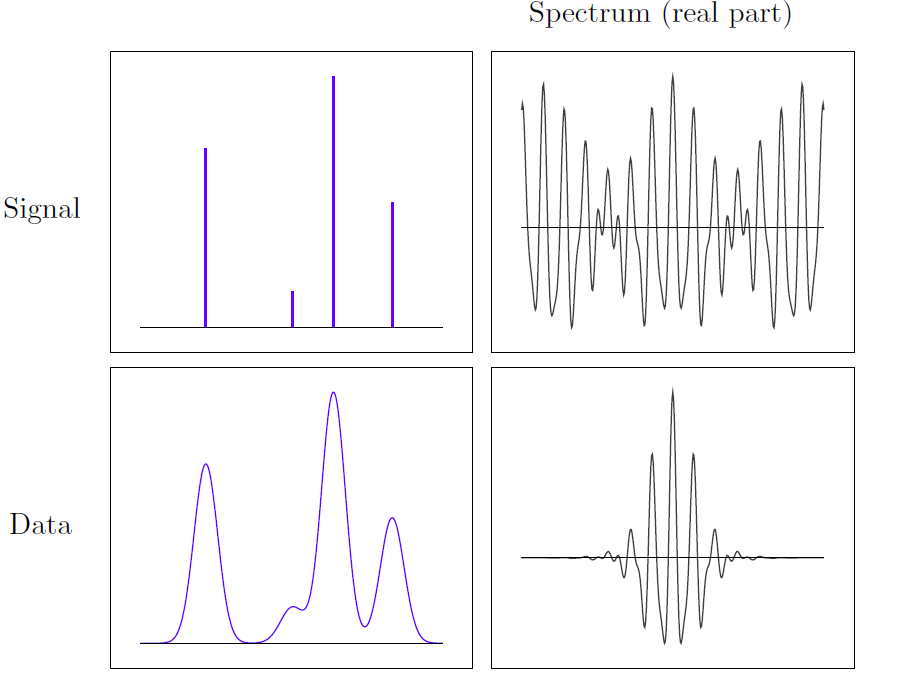
\includegraphics[width=0.7\textwidth]{../img/sig_data.png}
	\label{801}
	\caption{\textbf{Schematic of Super-Resolution.} The original signal and observed data for the super-resolution problem with their frequency spectra, as illustrated in \cite{fernandez2016super}.}
\end{figure}

In our setting, we assume the original data are a train of spikes, as shown in Figure~\ref{801}. Note that recovering the original signal from its low-pass observation without additional assumptions is an ill-posed problem, as the high-frequency component of the signal could be arbitrary. The necessary assumption for recovery turns out to be the intuitive property of a \emph{minimum separation} between spikes. Suppose the cut-off frequency of the observation filter is $f_c$. As illustrated in Figure 2 of \cite{fernandez2016super}, the existence of a purely high-frequency spike train with minimum separation $ \frac{1}{2}\lambda_c $ implies that the spectrum of the difference of two spike trains with separation $ \lambda_c $ can be made to lie entirely outside of the low-pass band with cutoff $ f_c $, whereby it is in principle impossible to distinguish those two signals. This phenomenon is known as the Rayleigh diffraction limit \cite{fernandez2016super}.

An interesting aspect of super-resolution that has been studied recently is the possibility of solving the recovery problem by convex relaxation techniques. Several works have been devoted to characterizing the accuracy and robustness to noise of different convex relaxations of the super-resolution problem \cite{candes2014towards,azais2015spike,duval2015exact,fernandez2013support,tang2015near}. In particular, \textsf{TV}-norm relaxation (a generalization of the $ \ell^1 $ norm to continuous domain) has been proven to successfully super-resolve spikes with minimum separation bounded by $ \approx 1.26\lambda_c $, although numerical experiments suggest that it in fact achieves the separation $\lambda_c$ described by the above heuristic reasoning.

In this work, we study convex relaxations of a generalization of the super-resolution problem to multiple observations where it is assumed that multiple independent spike trains are observed that all share the same support. This version of the problem was first described in \cite{fernandez2016super}. We propose a dual ceertificate that certifies the tightness of convex \textsf{gTV}-norm relaxation for this problem, as proposed in \cite{fernandez2016super}. Numerical experiments suggest that our certificate is dual-feasible up to the Rayleigh limit $\frac{1}{2}\lambda_c$, provided that the number of observations is large enough. We also discuss a theoretical approach to prove the feasibility of this dual certificate under suitable conditions on the minimum separation and number of observations, although the proof is left for future work.

\section{Formal Setup}

\subsection{Single Observation Problem Statement}

Suppose we observe a true signal whose representation in the physical domain is
\begin{equation}
    x^*(t) = \sum_{j = 1}^s a_j \delta_{t_j}(t),
\end{equation}
for $t \in \TT$ where $\TT = \RR / \ZZ$, which we will usually think of as the unit interval $[0, 1]$ with its endpoints identified, and $T = \{t_j\}_{j = 1}^s \subset \TT$ a discrete support set.
In the Fourier domain, this signal takes the form
\begin{equation}
    \widehat{x^*}(k) = \sum_{j = 1}^s a_j \exp(-2\pi i k t_j)
\end{equation}
for $k \in \ZZ$.

Now, we are interested in recovering this true signal $x$ from an observation that suffers from low resolution, which we represent as convolution of $x(t)$ with a point-spread function (PSF) denoted by $\phi(t)$.
We then observe the signal
\begin{equation}
    (\phi * x^*)(t) = \sum_{j = 1}^sa_j \phi(t - t_j).
\end{equation}
In the simplest case, $\phi$ is a Dirichlet kernel with cutoff frequency $f_c$, in which case the Fourier transform of the above is simply the truncation of the Fourier transform of $x^*$.
Denoting by $y$ the signal we observe in the Fourier domain, we have
\begin{equation}
    y(k) = \left(\sum_{j = 1}^s a_j \exp(-2\pi i k t_j)\right)\One\{|k| \leq f_c \}.
\end{equation}
We may then think of the data we observe as simply the $2f_c + 1$ values $y(-f_c), \dots, y(f_c)$.
We write $\sF_n$ for the sensing operator mapping $x^*$ to these $n$ Fourier coefficients.
A popular technique for solving this problem is \emph{total variation minimization}, which attempts to recover $x^*$ by solving the convex problem
\begin{equation}
    \mathrm{minimize} \HS \|x\|_{\mathsf{TV}} \HS \mathrm{subject\ to} \HS \sF_nx = y.
\end{equation}

\subsection{Extension to Multiple Observations}

We now consider a generalization of the problem presented in the previous section, where we make \emph{several} observations signals sharing the support $T = \{t_1, \dots, t_s\}$ of $x^*$, but having varying amplitudes $a_j$.
To formalize this, our true signal is now
\begin{equation}
    x^*_\ell(t) = \sum_{j = 1}^s a_{\ell, j} \delta_{t_j} \text{ for } \ell \in \{1, \dots, m\},
\end{equation}
and our observations are $y_{\ell, k} = (\sF_n x^*_\ell)_{k}$ for $k \in \{-f_c, \dots, f_c\}$ and $\ell \in \{1, \dots, m\}$.
We think of the $a_{\ell, j}$ as organized into vectors $\ba_{j} \in \RR^m$ for $j \in \{1, \dots, s\}$, and the  $y_{\ell, k}$ as organized into a matrix $\bY \in \CC^{m \times n}$.
The \emph{group total variation minimization} is the natural extension of the previous convex problem to this setting, where we solve
\begin{equation}
    \mathrm{minimize} \HS \|x\|_{\mathsf{gTV}} \HS \mathrm{subject\ to} \HS \left[\begin{array}{cccc}\sF_nx_1 & \sF_n x_2 \cdots \sF_n x_m \end{array}\right]^\top = \bY.
\end{equation}

\subsection{Dual Certificates}

In this section, we briefly describe the results of applying Lagrangian duality to \textsf{TV} and \textsf{gTV} norm minimization, the main tool for theoretical analysis of the performance of these algorithms.

\begin{definition}
    Let $\mu^0 \subset \CC$ denote the complex unit circle.
    A \emph{sign pattern} on a set is an assignment of points of $\mu^0$ to each point of the set.
\end{definition}

\begin{definition}
    For a sign pattern $v \in (\mu^0)^T$, a low-pass trigonometric polynomial $q: \TT \to \CC$,
    \begin{equation}
        q(t) = \sum_{k = -f_c}^{f_c} c_k e^{2\pi i k t},
    \end{equation}
    is a \emph{single-observation dual certificate} for $v$ if $q(t_j) = v_j$ for $t_j \in T$ and $|q(t)| < 1$ for $t \notin T$.
\end{definition}
\begin{proposition}[\textsf{TV} Norm Minimization Duality]
If a dual certificate for the sign pattern $v_j = a_j / |a_j|$ exists, then $x^*$ is the unique solution of \textsf{TV} minimization for the super-resolution problem.
\end{proposition}
Therefore, to prove the effectiveness of \textsf{TV} minimization it suffices to show that a dual certificate exists under some conditions on $T$.
The main result of \cite{fernandez2016super} establishes that this is true under a minimum separation condition.
\begin{definition}
    The \emph{minimum separation} of a set $T \subset \TT$ is
    \[ \Delta(T) = \min_{\substack{s, t \in T \\ s \neq t}} | s - t |, \]
    where we measure the wrap-around distance as on a circle.
\end{definition}

\begin{theorem}[Proposition 2.3 of \cite{fernandez2016super}]
    If $\Delta(T) \geq 1.26\lambda_c$ and $f_c \geq 10^3$, then a dual certificate exists for any sign pattern on $T$.
    \label{thm:single-obs-recovery}
\end{theorem}

As also observed in \cite{fernandez2016super}, the same ideas extend to the multiple observation case in a straightforward fashion.
\begin{definition}
    Let $\mu^{m - 1} \subset \CC^m$ denote the $m$-dimensional complex unit sphere.
    A \emph{$m$-dimensional sign pattern} on a set is an assignment of points of $\mu^{m - 1}$ to each point of the set.
\end{definition}
\begin{definition}
    For a sign pattern $\bv \in (\mu^{m - 1})^T$, a low-pass trigonometric polynomial $q: \TT \to \CC^m$ given by $q(t) = (q_1(t), \dots, q_m(t))$ and
    \begin{equation}
        q_\ell(t) = \sum_{k = -f_c}^{f_c} c_k \exp(2\pi i k t) \text{ for } \ell \in \{1, \dots, m\}
    \end{equation}
    is an \emph{$m$-observation dual certificate} for $v$ if $q(t_j) = \bv_j$ for $t_j \in T$, and $\|q(t)\|_{\ell^2} < 1$ for $t \notin T$.
\end{definition}
\begin{proposition}[\textsf{gTV} Norm Minimization Duality]
    If a dual certificate for the sign pattern $\bv_j = \ba_{j} / \|\ba_{j}\|_{\ell^2}$ exists, then $x^*$ is the unique solution of \textsf{gTV} minimization for the super-resolution problem.
\end{proposition}
However, while numerical experiments in \cite{fernandez2016super} suggest that when the amplitude vectors $\ba_j$ are taken randomly then recovery is possible down to a lower critical minimum separation which accumulates at $\frac{1}{2}\lambda_c$ as $m \to \infty$, the same uniform argument cannot apply---indeed, it is always possible that the amplitudes $\ba_j$ are all identical, in which case clearly it cannot be possible to recover $x^*$ any more effectively than in the one observation case.
Thus, to show that \textsf{gTV} norm minimization substantially improves on \textsf{TV} norm minimization, it is necessary to make some incoherence assumptions about the data generating process of the $\ba_j$.
One simple such assumption that captures the idea of these points being in ``general position'' is to assume that the signs $\ba_j / \|\ba_j\|_{\ell^2}$ are isotropically random unit vectors.

\section{Dual Certificate Construction}

Recall that we are interested in building a low-pass trigonometric polynomial $q: \TT \to \CC^m$ interpolating the points $(t_j, v_j)$ while remaining strictly inside the unit sphere in $\CC^m$ elsewhere.
The idea of the construction of \cite{fernandez2016super} when $m = 1$ is to build $q$ via kernel interpolation, and adjust it so that $q^\prime(t_j) = 0$ for each $j$, which one would hope might encourage the polynomial to remain in the unit sphere (in particular, this solves a problem with the naive approach of building an interpolant directly, where the polynomial does not remain inside the sphere near interpolated points but rather very slightly escapes).

The naive extension of this to the $m$-dimensional case is to require $q^\prime(t_j) = 0$ for each $t_j$.
However, numerical experiments show that the regime where this construction succeeds essentially does not depend on $m$, which is not surprising---after all, this is very close to just repeating the one-dimensional construction in each coordinate.
In this section, we propose a different dual certificate, which does appear to succeed numerically in certifying reconstruction down to the Rayleigh limit as $m \to \infty$.

\subsection{Step 1: Relaxing the Derivative Condition}

The first observation is that the condition $q^\prime(t_j) = 0$ is overkill for encouraging $q$ to remain in the unit sphere.
Intuitively, all that is really necessary is that $q^\prime(t_j)$ not have a component pointing out of the sphere, i.e.\ in the direction of $\bv_j$.
Thus, a reasonable condition is to require $q^\prime(t_j)$ and $\bv_j$, viewed as vectors, to be orthogonal.
However, it is not possible to express this constraint in complex arithmetic, so we must rewrite the dual certificate in terms of its real and complex parts (each of which is still low-pass).

Thus, we write $q_\ell(t) = q_\ell^R(t) + iq_\ell^I(t)$ for real-valued low-pass trigonometric polynomials $q_\ell^R$ and $q_\ell^I$.
We combine these into a single real-valued $2m$-dimensional trigonometric polynomial,
\begin{equation}
    \tilde{q}(t) = (q_1^R(t), q_1^I(t), \dots, q_m^R(t), q_m^I(t)) \in \RR^{2m}.
\end{equation}
Likewise writing $v_{j, \ell} = v_{j, \ell}^R + iv_{j, \ell}^I$ and $\tilde{\bv}_j = (v_{j, 1}^R, v_{j, 1}^I, \dots, v_{j, m}^R, v_{j, m}^I)$, we can express the interpolation conditions that the dual certificate $q$ must satisfy in terms of these new variables in essentially the same way: $\tilde{q}(t_j) = \tilde{\bv}_j$ for $j \in \{1, \dots, s\}$, and $\|\tilde{q}(t)\|_{\ell^2} < 1$ for all $t \notin T$.
We can also now formulate the conditions we will require of our interpolant.
\begin{enumerate}[leftmargin=1.8cm]
\item[\textsf{INT1}.] $\tilde{q}(t_j) = \tilde{\bv}_j$ for $j \in \{1, \dots, s\}$.
\item[\textsf{INT2}.] $\la \tilde{q}^\prime(t_j), \tilde{\bv}_j \ra = 0$ for $j \in \{1, \dots, s\}$.
\end{enumerate}

\subsection{Step 2: Kernel Interpolation}

We now proceed just as in \cite{fernandez2016super}, viewing the problem constructed in the previous section as a purely real-valued one: fix a real-valued low-pass kernel $K$, and define
\begin{equation}
    \tilde{q}_{\ell}(t) = \sum_{j = 1}^s \alpha_{j, \ell}K(t - t_j) + \sum_{j = 1}^s \beta_{j, \ell} K^\prime(t - t_j)
    \label{eq:interpolant-def}
\end{equation}
for $\ell \in [2m]$ and coefficients $\alpha_{j, \ell}, \beta_{j, \ell} \in \RR$ to be determined.
We think of these as organized into vectors $\balpha, \bbeta \in \RR^{2sm}$ where the entries are written iterating first over $j$, then over $\ell$ (in ``row major'' order).
To concisely write conditions \textsf{INT1} and \textsf{INT2} from the previous part, we first make a small definition.
\begin{definition}
    For a function $K: \TT \to \RR$ and an ordered point set $T = \{t_1, \dots, t_s\} \subset \TT$, define $\bD(K, T) \in \RR^{s \times s}$ to have entries
    \begin{equation}
        (\bD(K, T))_{j, k} = K(t_j - t_k).
    \end{equation}
\end{definition}
We also define the vector $\tilde{\bv}$ to be the $\tilde{v}_{j, \ell}$ flattened, also in row-major order.
Conditions \textsf{INT1} and \textsf{INT2} may then be written as the matrix equation
\[ \left[ \begin{array}{cc} \bm I_{2m} \otimes \bD(K, T) & \bm I_{2m} \otimes \bD(K^\prime, T) \\ (\one_s\tilde{\bv}^\top) \odot (\one_{2m}^\top \otimes \bD(K^\prime, T)) & (\one_s \tilde{\bv}^\top) \odot (\one_{2m}^\top \otimes \bD(K^{\prime\prime}, T)) \end{array}\right]\left[\begin{array}{c}\balpha \\ \bbeta \end{array}\right] = \left[\begin{array}{cc} \tilde{\bv} \\ \bm 0 \end{array}\right]. \]
We set some notation for the matrix on the left-hand side and the blocks corresponding to the set of equality constraints and derivative constraints:
\[ \bA = \left[\begin{array}{c} \bA_{\eq} \\ \bA_{\der} \end{array}\right] = \left[ \begin{array}{cc} \bm I_{2m} \otimes \bD(K, T) & \bm I_{2m} \otimes \bD(K^\prime, T) \\ (\one_s\tilde{\bv}^\top) \odot (\one_{2m}^\top \otimes \bD(K^\prime, T)) & (\one_s \tilde{\bv}^\top) \odot (\one_{2m}^\top \otimes \bD(K^{\prime\prime}, T)) \end{array}\right]. \]

\subsection{Step 3: Choosing Solution of Underconstrained System}

Note that the system described in the previous section has $4sm$ variables but only $2sm + s = (2m + 1)s$ constraints.
When the sign pattern is purely real, this reduces to $2s$ variables and $2s$ constraints, so there is (generically) a unique solution, as in the construction treated in \cite{fernandez2016super}.
In our more general setting, however, uniqueness typically fails, and so we must build a criterion for choosing a solution.

This extra freedom lets us further encourage $q(t)$ to remain inside the unit sphere.
In particular, a natural quantity to minimize is the $L^2$ norm of $q(t)$:
\begin{equation}
    \|q\|_{L^2(\TT)}^2 = \int_0^1 \|q(t)\|_{\ell^2}^2 dt.
\end{equation}
The added benefit of this choice is that it is a quadratic form in terms of the coefficients $\balpha, \bbeta$, so its minimization subject to linear constraints has a convenient closed form.
We now develop some notation to write down this quadratic form.
\begin{definition}
    For real-valued functions $K_1, K_2 \in L^2(\TT)$ and an ordered point set $T = \{t_1, \dots, t_s\} \subset \TT$, define $\bG(K_1, K_2, T) \in \RR^{s \times s}$ to have entries
    \begin{equation}
        (\bG(K_1, K_2, T))_{j, k} = \int_0^1 K_1(t - t_j)K_2(t - t_k)dt.
    \end{equation}
\end{definition}
Now, the $L^2$ norm of the polynomial $q(t)$ as defined in \eqref{eq:interpolant-def} is given by
\begin{align}
  \|q\|_{L^2(\TT)}^2
  &= \sum_{\ell = 1}^{2m} \sum_{j = 1}^s \sum_{k = 1}^s \bigg(\alpha_{\ell, j} \alpha_{\ell, k} \la K(\bullet - t_j), K(\bullet - t_k) \ra
    + \beta_{\ell, j} \beta_{\ell, k} \la K^\prime(\bullet - t_j), K^\prime(\bullet - t_k) \ra \\
    &\HS\HS\HS +\alpha_{\ell, j} \beta_{\ell, k} \la K(\bullet - t_j), K^\prime(\bullet - t_k) \ra\bigg)
  \nonumber \\
  &= \left[\begin{array}{c} \balpha \\ \bbeta \end{array}\right]^\top \left[\begin{array}{cc} \bm I_{2m} \otimes \bG(K, K, T) & \bm I_{2m} \otimes \bG(K, K^\prime, T) \\ \bm I_{2m} \otimes \bG(K^\prime, K, T) & \bm I_{2m} \otimes \bG(K^\prime, K^\prime, T) \end{array}\right]\left[\begin{array}{c} \balpha \\ \bbeta \end{array}\right].
\end{align}
We set a notation for the inner matrix:
\begin{align}
  \bG_0 &= \left[\begin{array}{cc} \bG(K, K, T) & \bm \bG(K, K^\prime, T) \\  \bG(K^\prime, K, T) & \bG(K^\prime, K^\prime, T) \end{array}\right] \succeq 0, \\
  \bG &= \left[\begin{array}{cc} \bm I_{2m} \otimes \bG(K, K, T) & \bm I_{2m} \otimes \bG(K, K^\prime, T) \\ \bm I_{2m} \otimes \bG(K^\prime, K, T) & \bm I_{2m} \otimes \bG(K^\prime, K^\prime, T) \end{array}\right].
\end{align}
We may then concisely write down the full quadratic problem by which we will determine the coefficients $\balpha, \bbeta$ as follows:
\begin{equation}
  \mathrm{minimize} \HS\left[\begin{array}{c} \balpha \\ \bbeta \end{array}\right]^\top \bG \left[\begin{array}{c} \balpha \\ \bbeta \end{array}\right]
  \HS\mathrm{subject\ to}\HS \bA \left[\begin{array}{c} \balpha \\ \bbeta \end{array}\right] = \left[\begin{array}{c} \tilde{\bv} \\ \bm 0 \end{array}\right]. \label{eq:opt-problem}
\end{equation}

\subsection{Explicit Solution}

As mentioned previously, \eqref{eq:opt-problem} has a closed-form solution, which may be derived with a straightforward Lagrange multiplier calculation, similar to the usual derivation of linearly constrained least-squares (corresponding to the case $\bG = \bm I$).
In our setting, the coefficients $\balpha, \bbeta$ are given by
\[ \left[\begin{array}{c} \balpha \\ \bbeta \\ \bm \lambda \end{array}\right] = \left[ \begin{array}{cc} \bG & \bA^\top \\ \bA & \bm 0 \end{array}\right]^{-1}\left[ \begin{array}{c} \bm 0 \\ \tilde{\bv} \\ \bm 0 \end{array}\right] \]
where $\bm \lambda \in \RR^{(2m + 1)s}$ are the Lagrange multipliers introduced in the calculation.
(The vectors on either side belong to $\RR^{(6m + 1)s}$.)
Moreover, we may explicitly invert this block matrix, and dispose of the Lagrange multipliers to obtain the simpler formula
\begin{equation}
    \left[\begin{array}{c} \balpha \\ \bbeta \end{array}\right] = \bG^{-1}\bA^\top(\bA \bG^{-1} \bA^\top)^{-1} \left[\begin{array}{c} \tilde{\bv} \\ \bm 0 \end{array}\right].
    \label{eq:opt-closed-form}
\end{equation}
Formula \eqref{eq:opt-closed-form} will be the beginning of our subsequent analysis; the remaining task is to obtain a detailed understanding of the structure of the matrix on the right-hand side.

\section{Numerical Evaluation}

In this section, we present some numerical results illustrating the performance of this dual certificate construction as the parameter $m$ increases.
These should be compared to Figures 3 and 9 of \cite{fernandez2016super} to observe that the dual certificate is feasible (and therefore certifies recovery) in basically all cases where the \textsf{gTV} convex program itself successfully achieves recovery.

First, in Figure~\ref{fig:real-complex}, we compare the case $m = 1$ with the case $m = 2$, which is the difference between real and complex sign patterns, and see that our dual certificate indeed is feasible more often in the latter case.
Second, in Figure~\ref{fig:higher-m}, we consider higher values of $m$, and note that the improvement continues, and the minimum separation at which the dual certificate stops being feasible for large support sets appears to approach the Rayleigh limit of $\frac{1}{2}\lambda_c$ as $m \to \infty$.

\section{Proof Outline for Dual Feasibility}

The following is a brief sketch of the ideas in our proof-to-be of the feasibility of this dual certificate construction.
\begin{enumerate}
\item First, we argue that the $\balpha$ are close to $\tilde{\bv}$ and the $\bbeta$ are small.
    Based on \eqref{eq:opt-closed-form}, this follows from arguing that
    \[ \bG^{-1}\bA^\top (\bA\bG^{-1}\bA^\top)^{-1} \approx \left[
            \begin{array}{cc} \bm I_{2m} & \bullet \\
              \bm 0 & \bullet
            \end{array}\right], \]
    where the bullets indicate $s$ columns whose values do not affect the values of $\balpha$ and $\bbeta$.
    This should follow just by properties of the kernel $K$: since the kernel is localized near zero, $\bA$ and $\bG$ should both be roughly diagonal, or roughly Toeplitz with very quickly decaying values away from the main diagonal.
    A numerical example of this structure is presented in Figure~\ref{fig:gram-matrices}.
    (The block $\bA_{\der}$ may cause problems here, especially since it depends upon the random $\tilde{\bv}$, but it appears to only influence the right-most columns of this matrix, which do not affect the values of $\balpha$ and $\bbeta$).
    Moreover, since the $L^2$ norm of $K^\prime$ is much higher than that of $K$, $\bG^{-1}$ should be close to zero on the lower half of its diagonal, which ensures that the lower block of this matrix is close to zero as needed.
    Many of the relevant bounds for this calculation are already collected in \cite{fernandez2016super}.

\item Next, we argue that in a small neighborhood of the support points $t_j$, $q(t)$ satisfies the necessary bound $\|q(t)\|_{\ell^2} < 1$.
    As explained nicely in \cite{tang2013compressed} for the one-dimensional case, this can be done just by using the derivative condition and showing that the Hessian of $\|q(t)\|_{\ell^2}^2$ (or something analogous) is negative-definite, so that there is a local maximum of the magnitude and Taylor's theorem gives the result in a sufficiently small neighborhood.

\item Finally, we must bound $\|q(t)\|_{\ell^2}$ away from all of the support points.
    Here it is important to use our probabilistic assumption on the $\bv_j$: since they are distributed uniformly on the unit sphere, they are roughly orthogonal, and so the tails of kernels centered at each $\bv_j$ should not be able to align sufficiently well to create a large value of $q(t)$ away from the support points.
    The orthogonality intuition can be formalized in a few ways, depending on what sorts of bounds we end up needing, but the most useful would probably be that the Gram matrix of the $\bv_j$ is distributed like a Wishart matrix normalized by the norms of Gaussian vectors (which concentrate tightly), so associated random matrix results can help bound its off-diagonal entries, which are distributed like the inner products of the $\bv_j$.
\end{enumerate}

\clearpage
\begin{figure}[!h]
    \begin{center}
        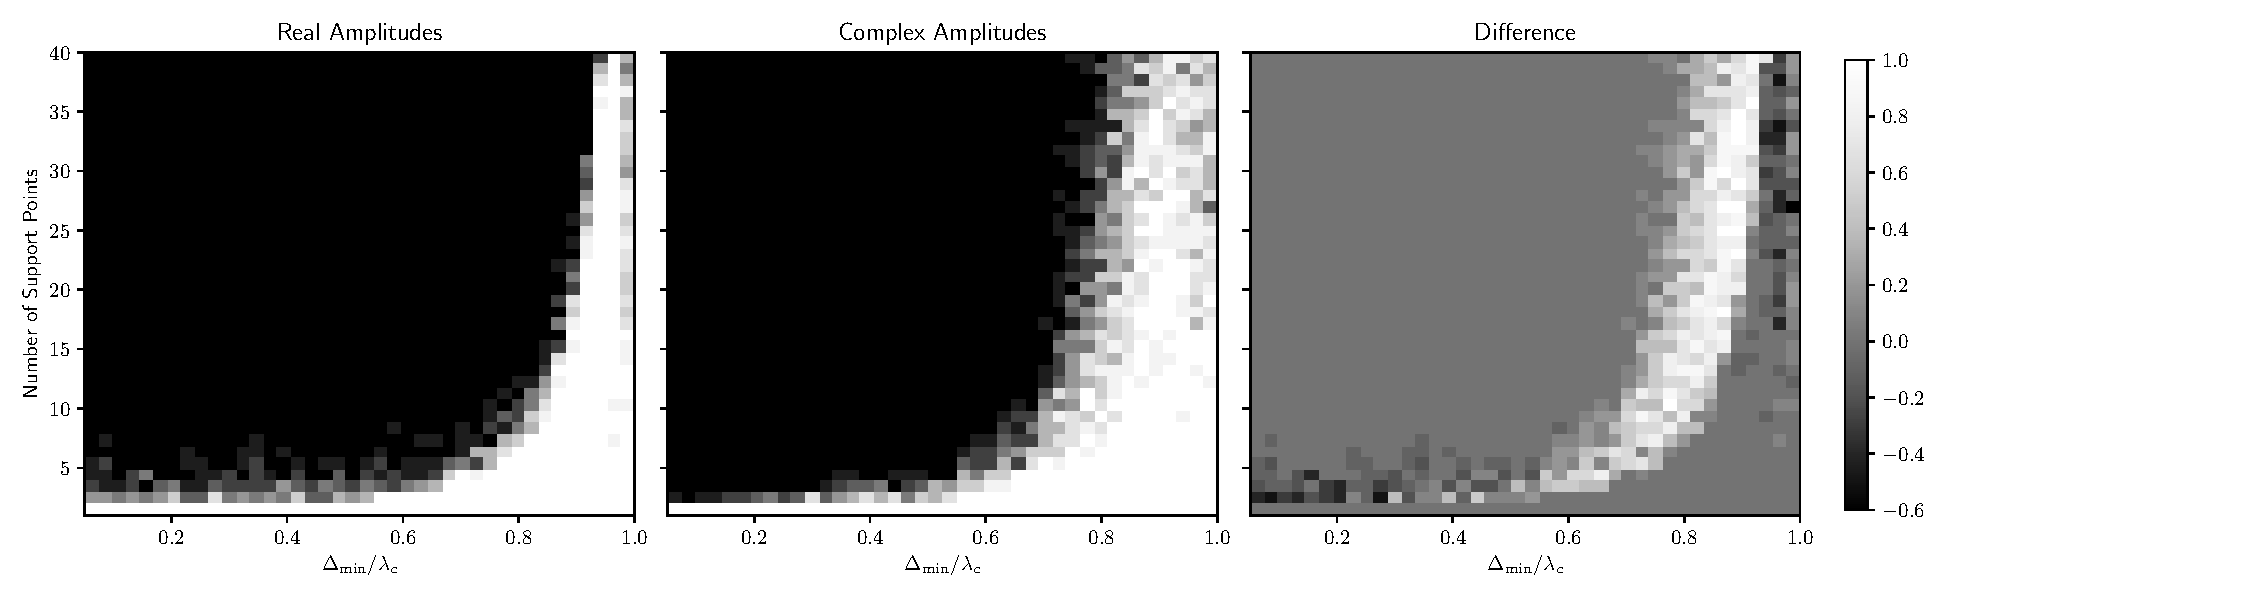
\includegraphics[trim={0 0 5cm 0},scale=0.5]{../img/real-vs-complex.pdf}
    \end{center}
    \vspace{-0.75cm}
    \caption{\textbf{Dual Certificate Feasibility: Real vs. Complex Amplitudes.} We show that our dual certificate construction performs better on random complex sign patterns than on random real sign patterns, showing the fraction of trials (out of 10) that the dual certificate is feasible in each case for fixed number of signals and minimum separation, and the difference between the fractions in the last panel.}
    \label{fig:real-complex}
\end{figure}
\begin{figure}[!h]
    \begin{center}
        \hspace{-0.6cm}
        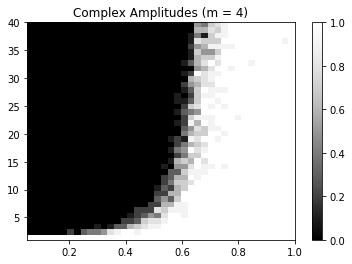
\includegraphics[scale=0.5]{../img/results-m=4.png}
        \HS \HS \HS
        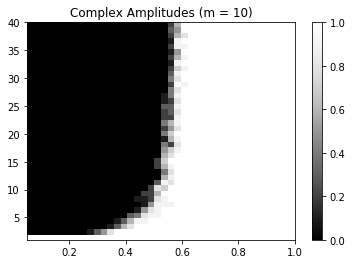
\includegraphics[scale=0.5]{../img/results-m=10.png}
    \end{center}
    \vspace{-0.75cm}
    \caption{\textbf{Dual Certificate Feasibility: Increasing Dimension.} We show that the trend of improving feasibility performance as $m \to \infty$ continues for higher values of $m$, with the feasibility phase transition appearing to saturate around a minimum separation of $\frac{1}{2}\lambda_c$.}
    \label{fig:higher-m}
\end{figure}
\begin{figure}[!h]
    \begin{center}
        \hspace{-3.5cm}
        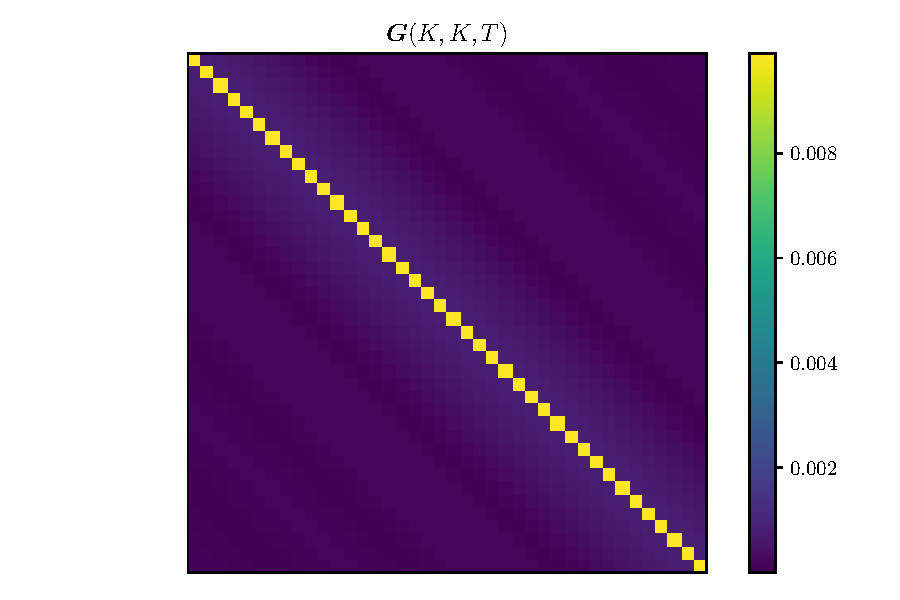
\includegraphics[trim={0 0 0 0},scale=0.5]{../img/kernel-gram.pdf}
        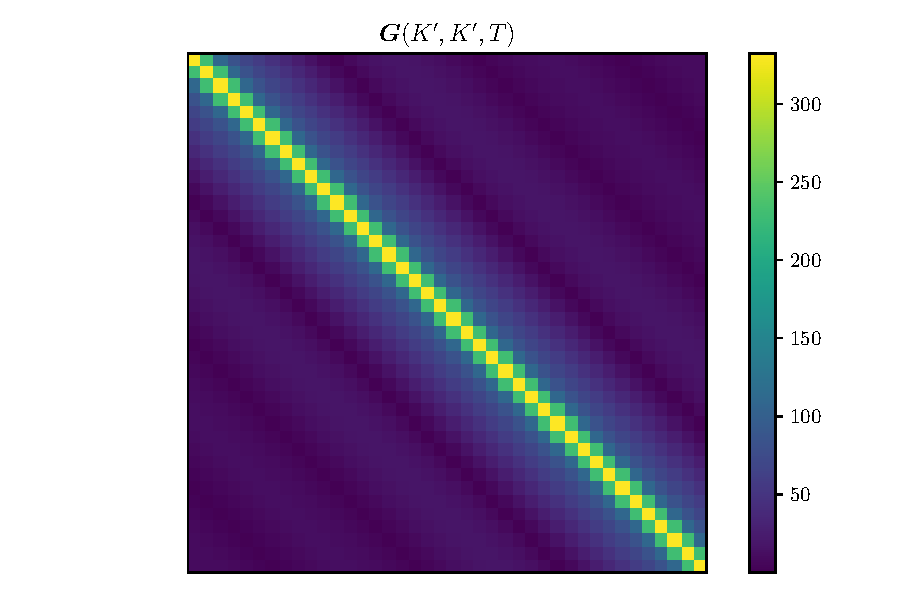
\includegraphics[trim={1cm 0 5cm 0},scale=0.5]{../img/kernel-derivative-gram.pdf}
    \end{center}
    \vspace{-0.75cm}
    \caption{\textbf{Shifted Kernel Gram Matrices.} We show the structure of Gram matrices of almost-regular shifts of a Dirichlet kernel, which are approximately Toeplitz with dominant diagonal values.
      The same for the kernel's derivative exhibits poorer decay and much higher values.}
    \label{fig:gram-matrices}
\end{figure}

\clearpage

\nocite{*}
\bibliographystyle{unsrt}
\bibliography{main}

\end{document}
%%% Local Variables:
%%% mode: latex
%%% TeX-master: t
%%% End:
